\chapter{Introducción}
\label{ch:intro}

Durante muchos años, ciberdelincuentes de todo el mundo se han servido de un gran número de tipos de ataques, generalmente, con la intención de lucrarse a costa de las víctimas o de, directamente, ``sembrar el caos'' (aunque puede haber más motivos); todo esto ha sido posible gracias a las vulnerabilidades que presentan los dispositivos informáticos, páginas web... En definitiva, elementos ``hackeables'' (\cite{historia-ciber}).%cita

Sin embargo, y en contraparte, grandes expertos en ciberseguridad y empleados de grandes empresas como Google o IBM han sabido solucionar los problemas que presentan estos dispositivos mediante, por ejemplo, parches en los programas informáticos... No obstante, las vulnerabilidades corregidas dan paso a otras potencialmente explotables y ello posibilita una mayor incidencia en el cibercrimen (Según \textit{FortiGuard Labs} de \textit{Fortinet}, el promedio de actividad semanal de ransomware en junio de 2021 fue más de 10 veces mayor que en 2020 \cite{guerra-ciber}).%cita

Y es de esta forma cómo se ha desarrollado este ``diálogo'' entre ambas partes desde, casi, los inicios de Internet inclusive. Sin embargo, con el paso del tiempo se han ido corrigiendo cada vez más cosas, y se está obligando a los ciberdelincuentes a ser más creativos con sus ataques: técnicas de phishing usando ingeniería social (\cite{phishing}), ataques a cadenas de suministro (\cite{cadena-suministro}), archivos con malware introducido en su interior (\cite{malware-imagen}), entre otras. %cita %cita %cita

A pesar de que existen muchos tipos de ataques, nos vamos a centrar en aquellos que utilizan archivos con malware introducido en su interior mediante \textbf{esteganografía}. Concretamente, trataremos de solucionar el problema que conlleva usar la herramienta Stegosploit (\cite{stegosploit}). Stegosploit es una herramienta que permite a un atacante introducir código malicioso (como un exploit de una vulnerabilidad) para ser ejecutado en el navegador de la víctima. Dependiendo de su uso, es posible que el atacante pueda infectar el equipo de la víctima con algún tipo de malware y que el mismo sea el objetivo de, por ejemplo, ``botnets'' \cite{botnet}.

Para evitar este tipo de incidencias, proponemos la utilización de un modelo de Deep Learning que pueda detectar el malware oculto dentro de las imágenes.

\section{Modelo para la detección de malware usando Deep Learning}

Como se puede apreciar en el capítulo \ref{ch:sota}, la mayoría de trabajos y revisiones adoptadas por la comunidad se han basado en Machine Learning y una pequeña parte en Deep Learning. De hecho, en muchos casos, se han obtenido buenos resultados en su detección, pero cabe destacar una observación muy importante: la mayoría de estos métodos basan su detección en información oculta, principalmente, en los \textbf{metadatos} del archivo.

Lo que proponemos con este trabajo es, mediante el uso de Deep Learning, crear un modelo capaz de detectar malware oculto en la misma imagen, es decir, en sus \textbf{datos}. Dicho de otra forma, pretendemos detectar malware oculto en imágenes a nivel de bit de datos.

Esto tampoco es nada nuevo, ya ha sido planteado dentro del capítulo \ref{ch:sota}, sin embargo ha sido desde una perspectiva con vistas a Machine Learning y no a Deep Learning.

El proceso que procederemos a ejecutar más adelante seguirá, grosso modo, la siguiente esquemática:

\begin{figure}[h]
  \centering
  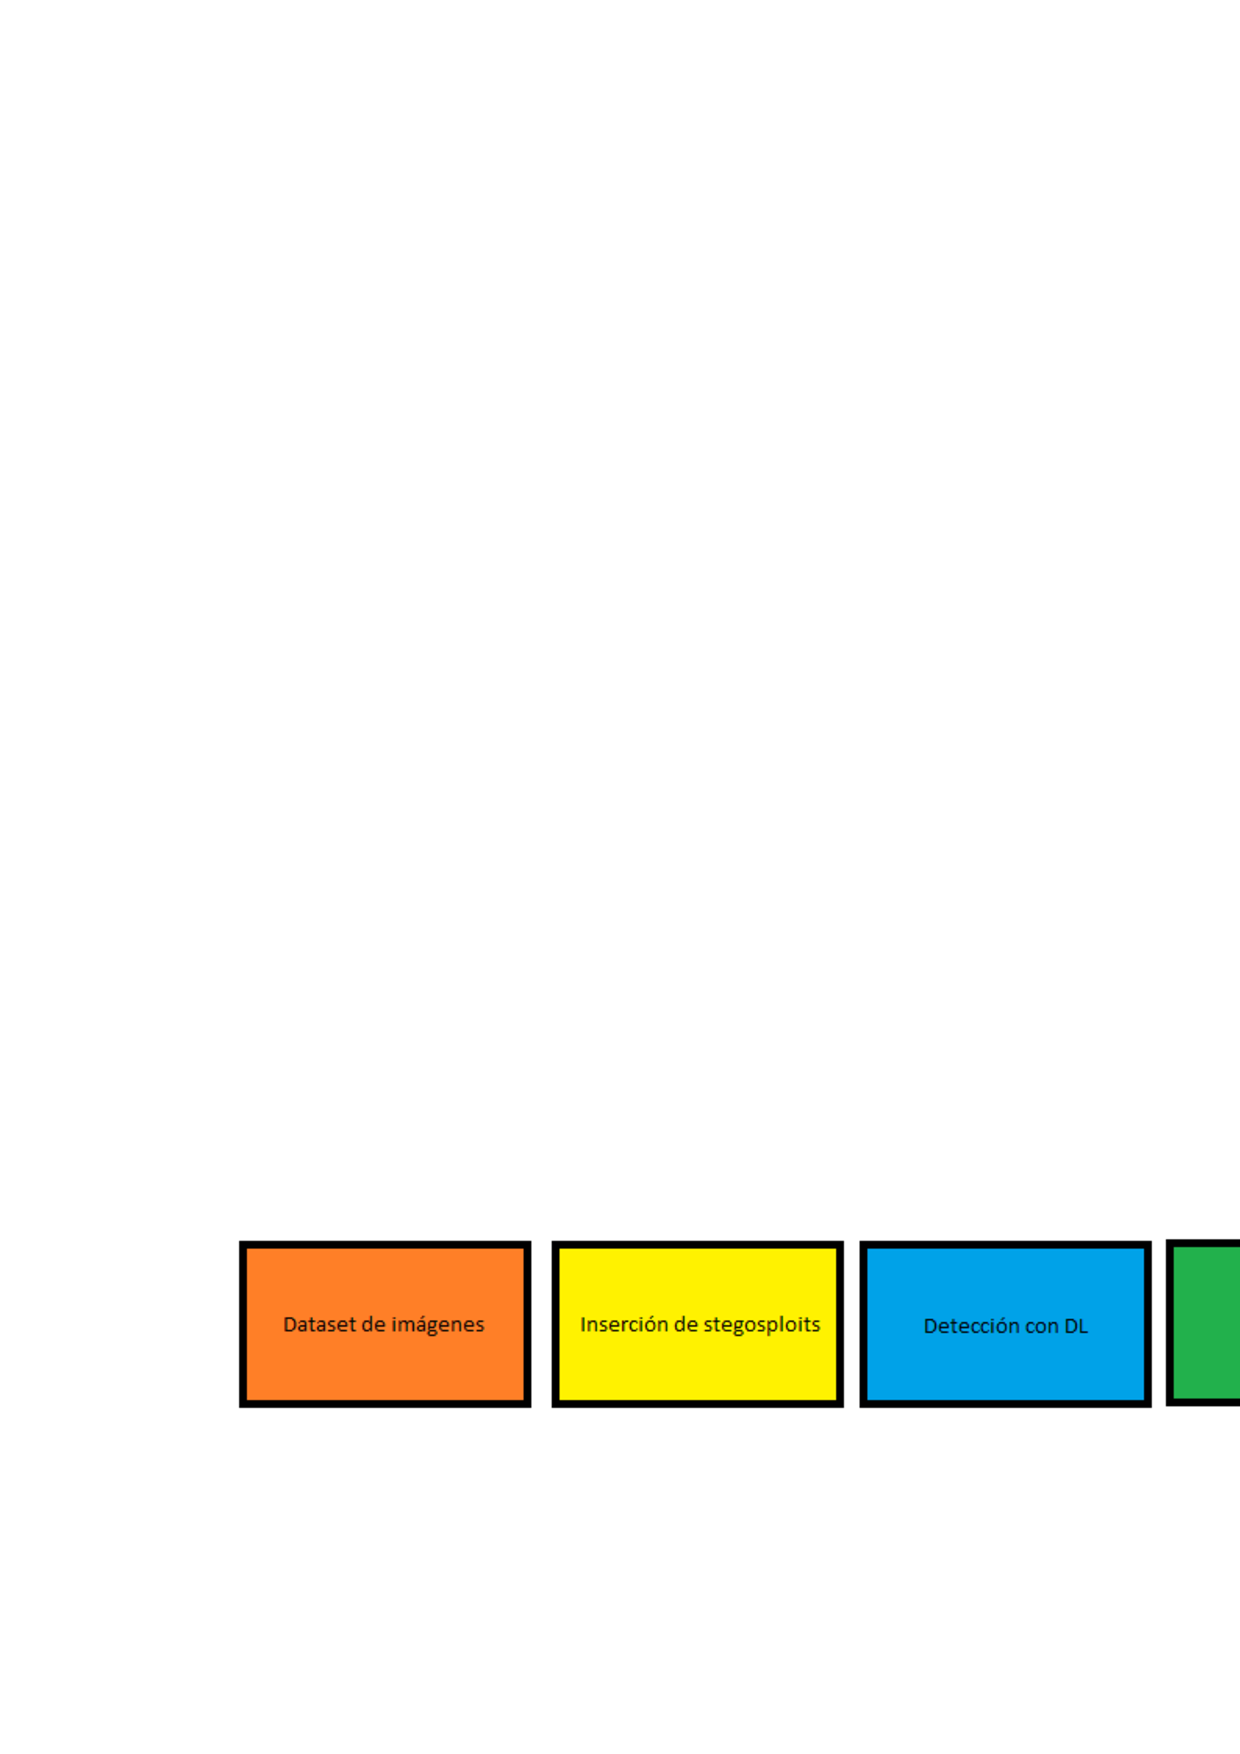
\includegraphics[width=16cm]{Figuras/Introduccion/Descripcion_Trabajo.png}
  \caption{Fases del proyecto}
  \label{fig:diagrama_bloques}
\end{figure}

Según la figura \ref{fig:diagrama_bloques}, comenzamos descargando un set de imágenes de Internet. Haciendo uso de la herramienta \textbf{Stegosploit}, de la que hablaremos más adelante, insertaremos malware dentro de los datos de algunas imágenes. Por último, aplicaremos diferentes modelos de Deep Learning para su detección dentro de todo el set. Más tarde, comentaremos los resultados.

\section{Objetivo principal}

El objetivo principal del proyecto es conseguir confeccionar un modelo de detección de malware oculto en imágenes mediante esteganografía, haciendo uso de herramientas de Deep Learning. Más concretamente:

\begin{itemize}
\item Trataremos de introducir código malicioso correctamente usando la herramienta Stegosploit y,
\item Trataremos de entrenar de forma eficaz una serie de modelos de Deep Learning para la detección de malware en imágenes.
\end{itemize}

Como ya hemos dicho anteriormente, los modelos creados para este fin se basan en tecnología Machine Learning, por ello esperamos que este trabajo sea uno de los primeros pasos en el largo camino que queda dentro de esta rama de investigación.

\section{Campos de aplicación}

Este trabajo será aplicable a cualquier ordenador con características apropiadas para la ejecución de tecnología Deep Learning en un tiempo adecuado. De este modo, facilitamos una solución para el uso diario del usuario en su tiempo de ocio o en su horario laboral; para las empresas en el caso de que se reciba por el correo electrónico corporativo una imagen maliciosa... En definitiva, una solución aplicable a una gran variedad de sectores y dominios. 

Dentro de las posibilidades que se presentan, podemos destacar las siguientes aplicaciones:
\begin{enumerate}
\item Implementación de soluciones avanzadas de detección de malware en imágenes.
\item Implementación de nuevas funciones de detección de malware en antivirus.
\item Desarrollo de nuevas tecnologías para facilitar la interacción de los usuarios de forma segura.
\end{enumerate}

\section{Organización del trabajo}

Este documento se organiza de la siguiente manera: en el siguiente capítulo hablaremos del estado del arte sobre los sistemas de detección de malware en imágenes para tener una idea clara de los avances que se han ido dando poco a poco durante los últimos años. En el capítulo \ref{ch:det_mal} explicaremos qué es la esteganografía digital (con una breve introducción histórica) y pasaremos a mostrar cómo se estructura nuestro modelo tras la revisión del estado del arte. En el capítulo \ref{ch:stego}, veremos el proceso que hemos seguido para poner en práctica el modelo propuesto utilizando la herramienta \textbf{Stegosploit} para introducir malware en imágenes (\cite{stegosploit}). Más tarde, en el capítulo de \ref{ch:res}, realizaremos una comparativa del sistema para diferentes modelos de Deep Learning usados en el anterior capítulo, y decidiremos cual es el mejor según las métricas usadas. Por último y para acabar, comentaremos las conclusiones finales de los resultados obtenidos en el capítulo anterior. %cita